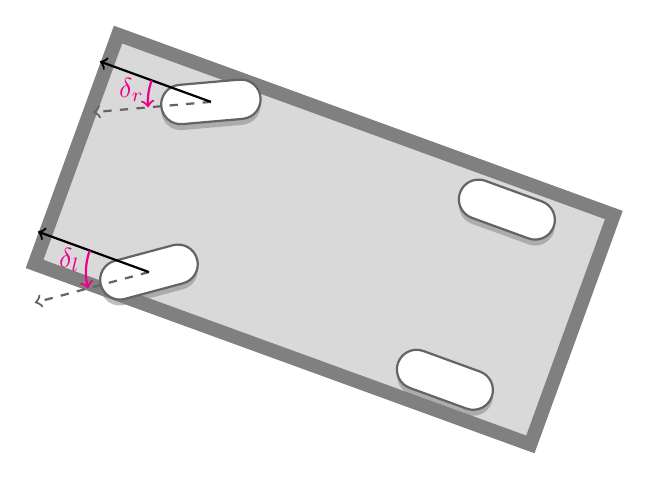
\begin{tikzpicture}[thick]
\usetikzlibrary{shapes.misc,shadows}
\usetikzlibrary{calc}
\usetikzlibrary{positioning,backgrounds}

\pgfmathsetmacro{\ArrowLength}{1}
\pgfmathsetmacro{\vheight}{4}
\pgfmathsetmacro{\vwidth}{2.3}
\pgfmathsetmacro{\deltavar}{35}
\pgfmathsetmacro{\deltavarB}{25}
\pgfmathsetmacro{\xdist}{8}

\pgfmathsetmacro{\voff}{1.5}
\definecolor{blue}{RGB}{100,100,100}

\pgfmathsetmacro{\myrot}{70}
\pgfmathsetmacro{\myshift}{1}
%\pgfmathsetmacro{\myrot}{0}
%\pgfmathsetmacro{\myshift}{0}
\begin{scope}[shift={(0,\myshift)},rotate=\myrot]


% RECTANGLE			
\draw [line width = 5, gray, fill=gray!30!white] (-0.4+\xdist,-1.3+\voff) rectangle (\xdist+\vwidth+0.4,\vheight+1.4+\voff);

% TIRES
%bottom left
\node(tire1)[draw=blue, thick, fill=white, 
			shape=rounded rectangle,  
			drop shadow={opacity=.5,shadow xshift=0pt},
			minimum width=1.5cm, 
			minimum height=0.5cm,
			rotate=90+\myrot]  at (\xdist,\voff)   {};

			
%top left
\node(tire2)[draw=blue, thick, fill=white, 
			shape=rounded rectangle,  
			drop shadow={opacity=.5,shadow xshift=0pt},
			minimum width=1.5cm, 
			minimum height=0.5cm,
			rotate=\deltavar-90+\myrot]  at (\xdist,\vheight+\voff)   {};
\draw[dashed, ->, blue]  (\xdist,\vheight+\voff)   --  ({\xdist-1.5*sin(\deltavar)},{\vheight+\voff+1.5*cos(\deltavar)}) ;

\draw[ ->]  (\xdist,\vheight+\voff)   --(\xdist,\vheight+\voff+1.5) ;
\draw[magenta,->] (\xdist,\vheight+\voff+0.8)  arc (90:90+\deltavar:0.8);
\node[magenta] at (7.8,6.5) {$\delta_l$};

%top right
\node(tire3)[draw=blue, thick, fill=white, 
			shape=rounded rectangle,  
			drop shadow={opacity=.5,shadow xshift=0pt},
			minimum width=1.5cm, 
			minimum height=0.5cm,
			rotate=\deltavarB-90+\myrot]  at (\xdist+\vwidth,\vheight+\voff)   {};

\draw[dashed, ->, blue]  (\xdist+\vwidth,\vheight+\voff)   --  ({\xdist+\vwidth-1.5*sin(\deltavarB)},{\vheight+\voff+1.5*cos(\deltavarB)}) ;


\draw[ ->]  (\xdist+\vwidth,\vheight+\voff)   --(\xdist+\vwidth,\vheight+\voff+1.5) ;
\draw[magenta,->] (\xdist+\vwidth,\vheight+\voff+0.8)  arc (90:90+\deltavarB:0.8);
\node[magenta] at (10.1,6.5) {$\delta_r$};

%bottom right
\node(tire4)[draw=blue, thick, fill=white, 
			shape=rounded rectangle,  
			drop shadow={opacity=.5,shadow xshift=0pt},
			minimum width=1.5cm, 
			minimum height=0.5cm,
			rotate=90+\myrot]  at (\xdist+\vwidth,\voff)   {};


			

%\draw[line width=2, color=blue]  (tire1.center) -- (tire2.center); 



\end{scope}




\end{tikzpicture}